\section{complex software development}

three most significant dimensions:  

\begin{itemize}
  \item requirements
  \begin{itemize}
    \item simple: one customer, one developer
    \item usually: stakeholders (glossary) with different needs that change, sometimes who start to understand what they want when they are
    provided with someone else’s impression of what they want.
  \end{itemize}
  \item technology
  \begin{itemize}
    \item simple tech rerly used in software development
    \item usually more than one piece is of need
  \end{itemize}
  \item people
  \begin{itemize}
    \item skills, intelligence levels, experience, viewpoints, attitudes, and prejudices, complexity level
    goes through the roof
  \end{itemize}
\end{itemize}

usually intersection between requirement complexity and tech complexity define the total complexity of a project. 

\begin{figure}[H]
  \centering
  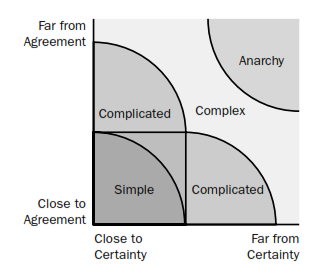
\includegraphics[width=0.6\textwidth]{./figures/chapter_1/complexity_assessment_graph.PNG}
  \caption{complexity assessment graph}
  \label{fig:ch1-complexity_assessment_graph}
\end{figure}\bigskip

The team takes a look at the requirements, considers the available technology, and evaluates its own skills and capabilities. It then collectively determines how to build the functionality.



